\section{Problemløsning}

[Indledning til overafsnittet problemløsning]

\subsection{Teknologier til visualisering}
Vi ser en tydelig mulighed for at assistere forbrugere med at træffe et valg, når det kommer til køb af varer på nettet. For at undersøge hvilke teknologier, der kan anvendes til visualisering, er der i dette afsnit en række teknologier og metoder, som alle er relevante i forhold til at visualisere en lampe. Teknologierne er udvalgt på baggrund af diskussion i gruppen, hvor mindre relevante teknologier, som f.eks. 3D-print blev fravalgt. Formålet med afsnittet er, at få en forståelse af hvilke teknologier der allerede eksisterer inden for visualisering, og finde ud af hvilke metoder, der er bedst i forhold til visualisering af lamper for brugere der handler via internettet.

\subsubsection{Digitale billeder taget med et fysisk kamera}
Som beskrevet under afsnit \ref{sec:ehandel}, benytter e-butikker, sig ofte af billeder til at vise kunden deres varer over internettet. Et eksempel på dette er vist på figur \ref{fig:e_handel_lampebilleder}.

\begin{figure}[H]
    \centering
    \fbox{\rule{\textwidth}{5cm}}
    \caption{Billeder af lamper på e-butikken somelampstore.what}
    \label{fig:e_handel_lampebilleder}
\end{figure} 

I det viste tilfælde er visualiseringen skabt ved at tage billeder af lamperne med et kamera fra en bestemt vinkel, i en kontekst, der typisk hænger sammen med lampetypen. 

Fordelen ved denne type af visualisering er, at den giver et virkelighedstro billede af, hvordan lampen ser ud i den kontekst, som billedet er taget i. Ulempen er, at der ofte kun er et begrænset antal billeder til rådighed, hvilket kan medføre, at forbrugeren ikke kan se lampen fra alle vinkler og på den måde ikke kan visualisere lampen for sig. Derudover kan det være svært, at se hvordan lyset udbreder sig fra lampen, da dette til dels afhænger af hvilken vinkel man ser lampen fra. 

Herudfra kan man kortfattet sige, at visualisering af lamper gennem billeder, taget med et fysisk kamera, giver et realistisk billede af lampen, men kun i den kontekst og vinkel billedet er taget i. 

% \subsubsection{3D print}
% En teknologi, som lampebutikker vil kunne bruge, er 3D printere. 3D printere anvender plastik istedet for blæk, som bliver varmet op til knap 200 grader \cite{hvordan_3Dprinter}. Den flydende plastik bliver lagt i tynde lag og størkner hurtigt efter at have bundet sig med det underliggende lag. 

% Sælgeren kan give forbrugeren en fil, så forbrugeren selv vil være i stand til at lave et 3D print af en bestemt lampe. Dette forudsætter dog, at forbrugeren har en 3D printer og, at brugeren er dedikeret nok til at få printet lampen, da store objekter kan tage dage at printe og ofte skal deles op i mindre dele.\cite{hvordan_3Dprinter}. Derudover er 3D printere stadig en så ny teknologi, og de er stadig primært rettet mod hobbyfolk som vil bruge lang tid på, at få kallibreret printeren korrekt, da et print ellers nemt kan fejle. 3D printer er heller ikke en billig inverstering, da nogle modeller koster over titusinde kroner\cite{3D_printer}. 

% Idag vil det være en dårlig ide for lampebutikker at forvente, at deres kunder har en 3D printer derhjemme. Et andet problem er, at lampebutikker også kommer i et dilemma, da lampebutikker skal bestemme om man kan udgive tegninger inden forbrugeren har købt lampen eller om de skal betale en form for depositum.

\subsubsection{Computergrafik}
I computergrafik, er en 3D model, en beskrivelse af objekters form og materiale.\cite{computergrafik_introduktion} Computergrafiske metoder kan bruges til at immitere hvordan lys interaktere med modellen og på den måde tegne et billede af modellen. Der eksisterer en mængde forskellige computergrafiske metoder, flere af hvilke kan bruges sammen med andre for, at opnå et mere realistisk eller effektivt resultat. Der findes flere produkter som kan visualisere produkter til salg på websites som f.eks. Cylindo\cite{Cylindo}. Men vi har ikke kendskab til at andre specialisere sig, eller markedsføre sig på nuværende tidspunkt med deres kompetencer med fokus på visualisering af lampers belysning.

\paragraph{Rasterisering}
er en metode til at visualisere miljøer med høj aktiv brugerinteraktion som f.eks. computerspil.\cite{rastarization} Metoden virker ved rent mattematisk at projektere modellen på et billedplan som repræsentere skærmen.\cite{rastarization}. Fordelen ved resterisering er at disse projektioner, kan foretages meget hurtigt af computerens grafikkort, som bygget specielt til formålet\cite{rastarization}. Dette kan dog mindske fleksibiliteten, og muligheden for mere avancerede visualisering, hvor der kræves refleksioner og refraktioner af lys, som ikke passer ind i den proces (graphics pipeline\cite{rastarization}, som de enkelte grafikkort danner billeder ud fra. 

\paragraph{Ray tracing}\cite{raytracing_for_begyndere} forsøger, nøjagtigt at simulere lys i et viretuelt miljø, i modsætning til rasterisering hvor hastighed er den primære faktor. Raytracing bygger fundementalt på at følge stråler af lys og bygge en model for hvordan de stråler interaktere med forskællige objekter og materialer. Der skælnes mellem to typer af raytracing: Forwards raytracing og backwards raytracing.

\subparagraph{Forwards raytracing}\cite{radiosity_by_wpi,radiosity_by_uob} er oftere kaldet radiosity og vil bliver reffereret til som sådan fremhenværende. Radiosity er hvad man kunne kalde en forwards raytracing metode. Her eksistere lyskilder ikke som specielle objekter i en 3D model, hvilket er tilfældet for de andre metoder, men her som objekter uden forskel fra de andre i modellen.

I radiosity modellen er alle flader betegnet med en absorbans faktor og en energi faktor. Absorbansen beskriver hvor meget af lys der rammer fladen der bliver absorberet. Absorberet lys hæver en flades energi og som i virkeligheden, afgives noget af den energi som lys, mens andet bliver omdannet til f.eks. varme. Lyskilder er således blot flader som starter med en mængde energi.

Radiosity er i stor grad blandt de mest tidskrævende metoder eftersom at den laver beregninger som ikke nødvendigvis bliver set i et billede. Dette muliggøre dog at visualisere en scene en gang og derefter at kunne se den fra mange vinkler eftersom at de ekstra udregninger allerede er gjort. Radiosity er derimod ikke designet til at håndtere fænomener som er afhængig af hvor man ser et objekt fra, så som refleksion og refraktion. Dvs. at radiosity ikke kan håndtere metalliske overflader eller semitransparente materialer. Til gengæld er Radiosity rigtig god til at simulere matte overflader og skygger.

\subparagraph{Backwards raytracing} er hvad man i almindelighed kalder raytracing og vil bliver reffereret til som sådan fremhenværende. Raytracing forsøger at simplificerer den fysiske model af lys ved at ignorere det lys som ikke rammer vores øjne. Raytracing er dog alligevel blandt de metoder som kendes for at kunne skabe de mest fotorealistiske renderinger. Dette gøres ved såkaldt \textit{backwards raytracing}, hvorved man følger en stråle fra øjet og ud mod 3D modellen, så tjekkes der for kollisioner mellem strålen og objekterne i modellen. Ved hver kollision kan man vælge at følge yderligere stråler som kan hjælpe med at udregne reflektioner eller komplekse skygger. Denne metoder står i modsætning til hvad man kalder \textit{forwards raytracing} som er den mere fysisk korrekte metode, hvor man følger stråler af lys fra hver lyskilde.

I forhold til rasterisering, tager raytracede billeder væsentligt længere tid at tegne, men komplekse lysfænomener som refleksioner og lys forvrængninger igennem semitransparante medier som vand(kaldet refraktion) er simple at beskrive for en raytracing algoritme, som kan tegne disse med realistisk precision. Nogle fænomener som bløde skygger kan også beskrives men jo flere typer fænomener og jo større realisme der kræves des længere tid tager det at tegne et billede, men raytracing tillader stor fleksabilitet.

\subsubsection*{Opsummering}
Billeder af den fysiske lampe er gode til akkurat at gengive lampen, men det er et problem at der ofte ikke er billeder nok fra forskællige vinkler, at billederne kun viser lampens form og ikke dens lys og at det er for besværligt at tage billeder af lampen med forskællige pærer for at vise forskællige farvetemperature og at det også er bbesværligt at udskifte den kontekst som lampen bliver vist i. 

Computergrafik kan nemt indlejres i en hjemmeside. Hvilken Computergrafisk teknik der er den korrekte er et case til case valg eftersom det helt afhænger af hvor meget fleksibilitet versus kvalitet der er nødvendigt. Rasterisering og radiosity kan begge implementeres på en måde hvorved der opnås et højt niveau af bruger interaktion som kan gøre værktøjet mere naturligt at anvende for forbrugeren. Eftersom at målet er at simulere lamper og ikke møbler som borde og stole, er langt mere komplekst at lave en god visualisation med rasterisering. Radiosity falder også til kort hvis der er behov for mere komplekse materialer som metalliske overflader eller f.eks. klar plast og glas. Billeder tegnet med raytracing kan tage lang tid at rendere, men der er mulighed for stor fleksibilitet og komplekse materialer er relativt simple at rendere. Med det grundlag vil rapporten fremadrettet arbejde med raytracing som metode til visualisering.

\subsection{Ide}

[Forklaring af ide]

\subsubsection{Skitse af ide til løsning}

[Forklaring af skitse]

\subsection{Ide}

I dette afsnit er der beskrevet en ide til løsningen af den endelige problemformulering. Ideen er resultatet af en diskussion i gruppen, hvor vi kom med ideer til løsninger, og herefter diskuterede fordele og ulemper ved de forskellige ideer. Formålet med afsnittet er at skitsere gruppens bud på den optimale løsning på problemet, og afsnittet er derfor udarbejdet med feedback fra forskellige lampebutikker. I slutningen af afsnittet vil der være en afgrænsning af løsningen som vil danne grundlag for den senere udvikling af en løsning.

Den løsning som gruppen har valgt at arbejde med er, "3D modeller af lamper med interaktion". Som beskrevet i problemanalysen har gruppen valgt at løse problemet når kunder handler på e-butikker. Tanken er derfor at implementere software på en e-butiks hjemmeside med henblik på at løse problemet for kunden.

\subsubsection{Skitse af løsning}

\begin{figure}[H]
   \centering
   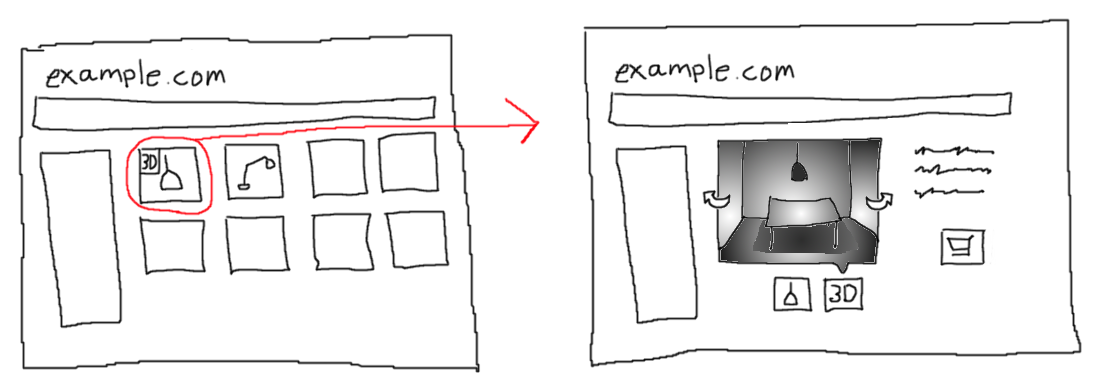
\includegraphics[width=\textwidth]{skitse_til_loesning}
   \caption{Skitse af ide til løsning.}
\end{figure}

På figur 5 er der illusteret en skitse af en e-butik som sælger lamper. Figuren illustrerer hvordan systemet kan integreres på en hjemmeside. Skitse 5a viser et online katalog over e-butikkens udvalg af lamper. Som der fremgår af skitsen vil nogle lamper være markeret med et "3D-ikon" og dette indikerer, at kunden har mulighed for, at se skitsen i 3D. Kunden tilgår 3D-billedet ved at klikke på ikonet. Når kunden trykker på ikonet bliver kunden omdirigeret til en anden menu. Som der fremgår af skitse 5b, så har kunden her mulighed for at se en 3D-model af lampen i et rum. De to pile på skitsen indikerer, at kunden har mulighed for at rotere billedet, og se hvordan belysningen fra lampen er, set fra forskellige vinkler. Som en ekstra feature har kunden mulighed for at indtaste en kontekst, beskrevet som en model, ind i programmet og har derefter mulighed for at se hvordan lampen ser ud i den kontekst som kunden ønsker. 
Derudover har kunden mulighed for, at justere lampens farvetemperatur (i kelvin), meningen med denne feature er, at kunden har mulighed for at visualisere hvordan forskellige pærer vil se ud i lampen. De forskellige 3D billeder vil ligge til rådighed på en ekstern server og vil derfor ikke gøre e-butikkernes hjemmeside betydeligt langsommere. Derudover er tanken af alle 3D billeder bliver udleveret af producenten af lamperne. 

\begin{figure}[H]
   \centering
   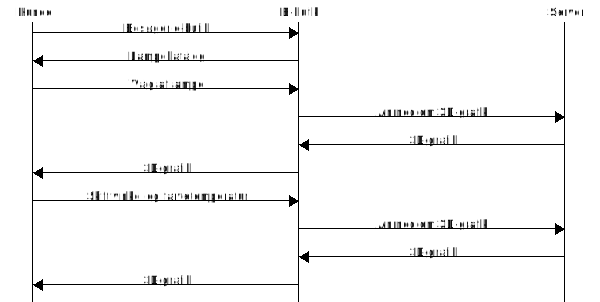
\includegraphics[width=\textwidth]{brugerinteraktion}
   \caption{Sekvensdiagram af løsningsideen.}
\end{figure}

Figur 6 tager udgangspunkt i en hjemmeside som har fået implementeret vores løsning, og viser et sekvensdiagram som illustrere processen når en kunde vil købe en lampe.  

I forbindelse med implementeringen af softwaren på en hjemmeside har der været forskellige ting som skulle overvejes. Da problemet omhandler visualisering af lys fra lamper, har gruppen valgt at fokusere på at lave en løsning hvis primære formål er at generere realistiske 3D-billeder af lamper. Disse billeder vil vise belysningen fra lamper med forskellige pærer. Features som interaktion og kontekst, har derfor anden priotet. 

Ud fra ovenstående beskrivelse har gruppen derfor valgt, i første omgang, at fokusere på at lave et program der gør det muligt for kunden, at visualisere hvordan lys spreder sig fra lamper illustreret igennem realistiske 3D-billeder. Derudover har kunden mulighed for at justere pærens farvetemperatur, og derved også se hvordan lampens belysning med forskellige pærer.  


\subsubsection{Krav til løsningen}

I forbindelse af vores projekt har vi fået nogle krav fra universitetets side. Disse er at programmet skal skrives i programmeringssproget C, derudover er der også tidsmæssigt pres da hele projektet kun varer ca.\ to en halv måned. 
Vi er også begrænset af vores egen viden indenfor emnet, da raytracing er en fremmed teknik, som få af os har haft tidligere erfaringer med. 

Vi har selv opstillet nogle krav til vores program for hvad vi mener programmet skal kunne før det kan være et færdigt produkt.
\begin{enumerate}
    \item Programmet skal kunne implementeres på en hjemmesiden (ellers bruges på en computer i den fysiske butik).
    \item skal kunne visualisere billedet relativt hurtigt, da kunderne ikke skal vente før de kan se billedet.
    \item Programmet skal kunne modtage et vilkårligt billede (i den rigtige format) og renderer dette.
    \item Lysets udbreddelse skal kunne ses tydeligt af kunden.
    \item Det skal være muligt for kunden skal kunne ændre farvetemperatur.
    \item Det skal være muligt for kunden at rotere billedet.
    \item Det skal være muligt for kunden at kunne indsætte en vilkårlig kontekst.
    \item Programmet skal være let at bruge, så en potentiel kunde ikke vil blive frusteret og derved vil forlade butikken/siden.
    \item 
\end{enumerate}

\subsubsection*{Opsummering}
[Kort opsummering af præcist ideen bag løsningen]

\subsubsection{Krav til løsningen}

[Krav/målsætninger for løsningen]

%\subsection{krav}

I forbindelse af vores projekt har vi fået nogle krav fra universitetets side. Disse er at programmet skal skrives i programmeringssproget C, derudover er der også tidsmæssigt pres da hele projektet kun varer ca to en halv måned. 
Vi er også begrænset af vores egen viden indenfor emnet, da raytracing er en fremmed teknik, som få af os har haft tidligere erfaringer med. 


\subsubsection*{Opsummering}

[Kort opsummering af præcist ideen bag løsningen]

\subsection{Teori}

[Beskrivelse af de teorier der skal anvendes i udviklingen løsningen]

\subsubsection{Vektorer i 3D}

[Beskrivelse af vektorer]

\subsubsection{Raytracing}

[Beskrivelse af raytracing]

\subsubsection*{Opsummering}

[Kort opsummerende beskrivelse af teorierne]

\subsection{Udvikling}

[Sammensætning af teorier igennem udviklingen af produktet, der løser problemet]

\clearpage